\documentclass{article}
\usepackage[left=3cm, right=3cm, top=2cm]{geometry}
\usepackage{amsmath}
\usepackage{amsfonts}
\usepackage{graphicx}
\usepackage{color}
\title{A Small \LaTeX{} Article Template\thanks{To your mother}}
\author{Your Name  \\
	Your Company / University  \\
	\and 
	The Other Dude \\
	His Company / University \\
	}

\date{\today}
% Hint: \title{what ever}, \author{who care} and \date{when ever} could stand 
% before or after the \begin{document} command 
% BUT the \maketitle command MUST come AFTER the \begin{document} command! 
\begin{document}
\vspace{-10pt}
In response to Comments 1-3 from \underline{Reviewer: 5 (Review30371)}. Following we mathematically and graphically analyze the proposed local behavior synergy extraction scheme which is composed of dimensionality reduction of the joint trajectories (via. PCA or K-PCA) and grouping of local behavior regions with GMM on this lower dimensional space. The $K$ clusters found in this embedded space correspond to the number of $K$ synergy matrices that will parametrize $\mathcal{A}(q)$. Let's begin by analyzing the proposed DS-based control-law:
\begin{equation}
\underbrace{\dot{q}}_{\mathbb{R}^{m\times 1}} = -\underbrace{\mathcal{A}(q)}_{\mathbb{R}^{m\times m}}\underbrace{J^{T}(q)}_{\mathbb{R}^{m\times d}}\underbrace{(H(q)-x^*)}_{\mathbb{R}^{d\times 1}}
\label{eq:jtds}
\end{equation}
The intuition behind this control-law is that $\mathcal{A}(q) = \sum\limits_{k=1}^{K}\theta(\phi(q))A_k$ is a linear combination of time-invariant linear matrices $A_k \in \mathbb{R}^{m \times m}$, \underline{these matrices are the ``local behavior synergy matrices"} that shape the motion in joint-space. Meaning that, given the joint-space velocity vector representing the task-space error $J^{T}(q)(H(q)-x^*)$, the resulting motion is biased to use a particular set of joints, defined in each $A_k$. Each $A_k$ is thus activated depending on the current ``joint-posture" $q$ (represented in the lower-dimensional space $\phi(q)$) via the scheduling/activation function $\theta(\phi(q))$. Hence, our proposed definition of ``local behavior synergies" is not analogous to the notion of ``hand posture synergies". 

Given the raw demonstrations of a joint-space  behavior with a task-space target as shown in Fig. \ref{fig:raw_demos} (for the pouring task) we seek to learn a linear combination of local behavior synergies $\mathcal{A}(q) = \sum\limits_{k=1}^{K}\theta(\phi(q))A_k$ such that we can use \eqref{eq:jtds} to accurately reproduce these demonstrations. In order to do so, we project the raw joint trajectories to a lower-dimensional space via $\phi(q)$, in the case of PCA $\phi(q)=M_p \times q$ for $M_p \in \mathbb{R}^{p \times m}$. By choosing the first 3 PCs we can explain 95\% of the variance in the joint posture trajectories, which can be represented in this 3-D space as shown in Fig. \ref{fig:raw_demos}. We then jointly learn the activation function $\theta(\cdot)$ and the number of $K$ local synergy regions by fitting a GMM to this representation of the joint posture trajectories. As can be seen in Fig. \ref{fig:raw_demos}, the entire joint-space motion can be represented by 3 local synergy regions in PCA-space. Meaning that we only need 3 synergy matrices $A_k$ to represent the complex joint-space motion accurately. The activation function $\theta(\cdot)$, as described in the mansucript, is the posterior probability of a joint posture in PCA-space $\phi(q)$ belonging to one of the local synergy regions $k \in \{1,\dots,K\}$.


\begin{figure*}[!th] 
  \begin{minipage}{0.58\textwidth}
     	\centering 
     	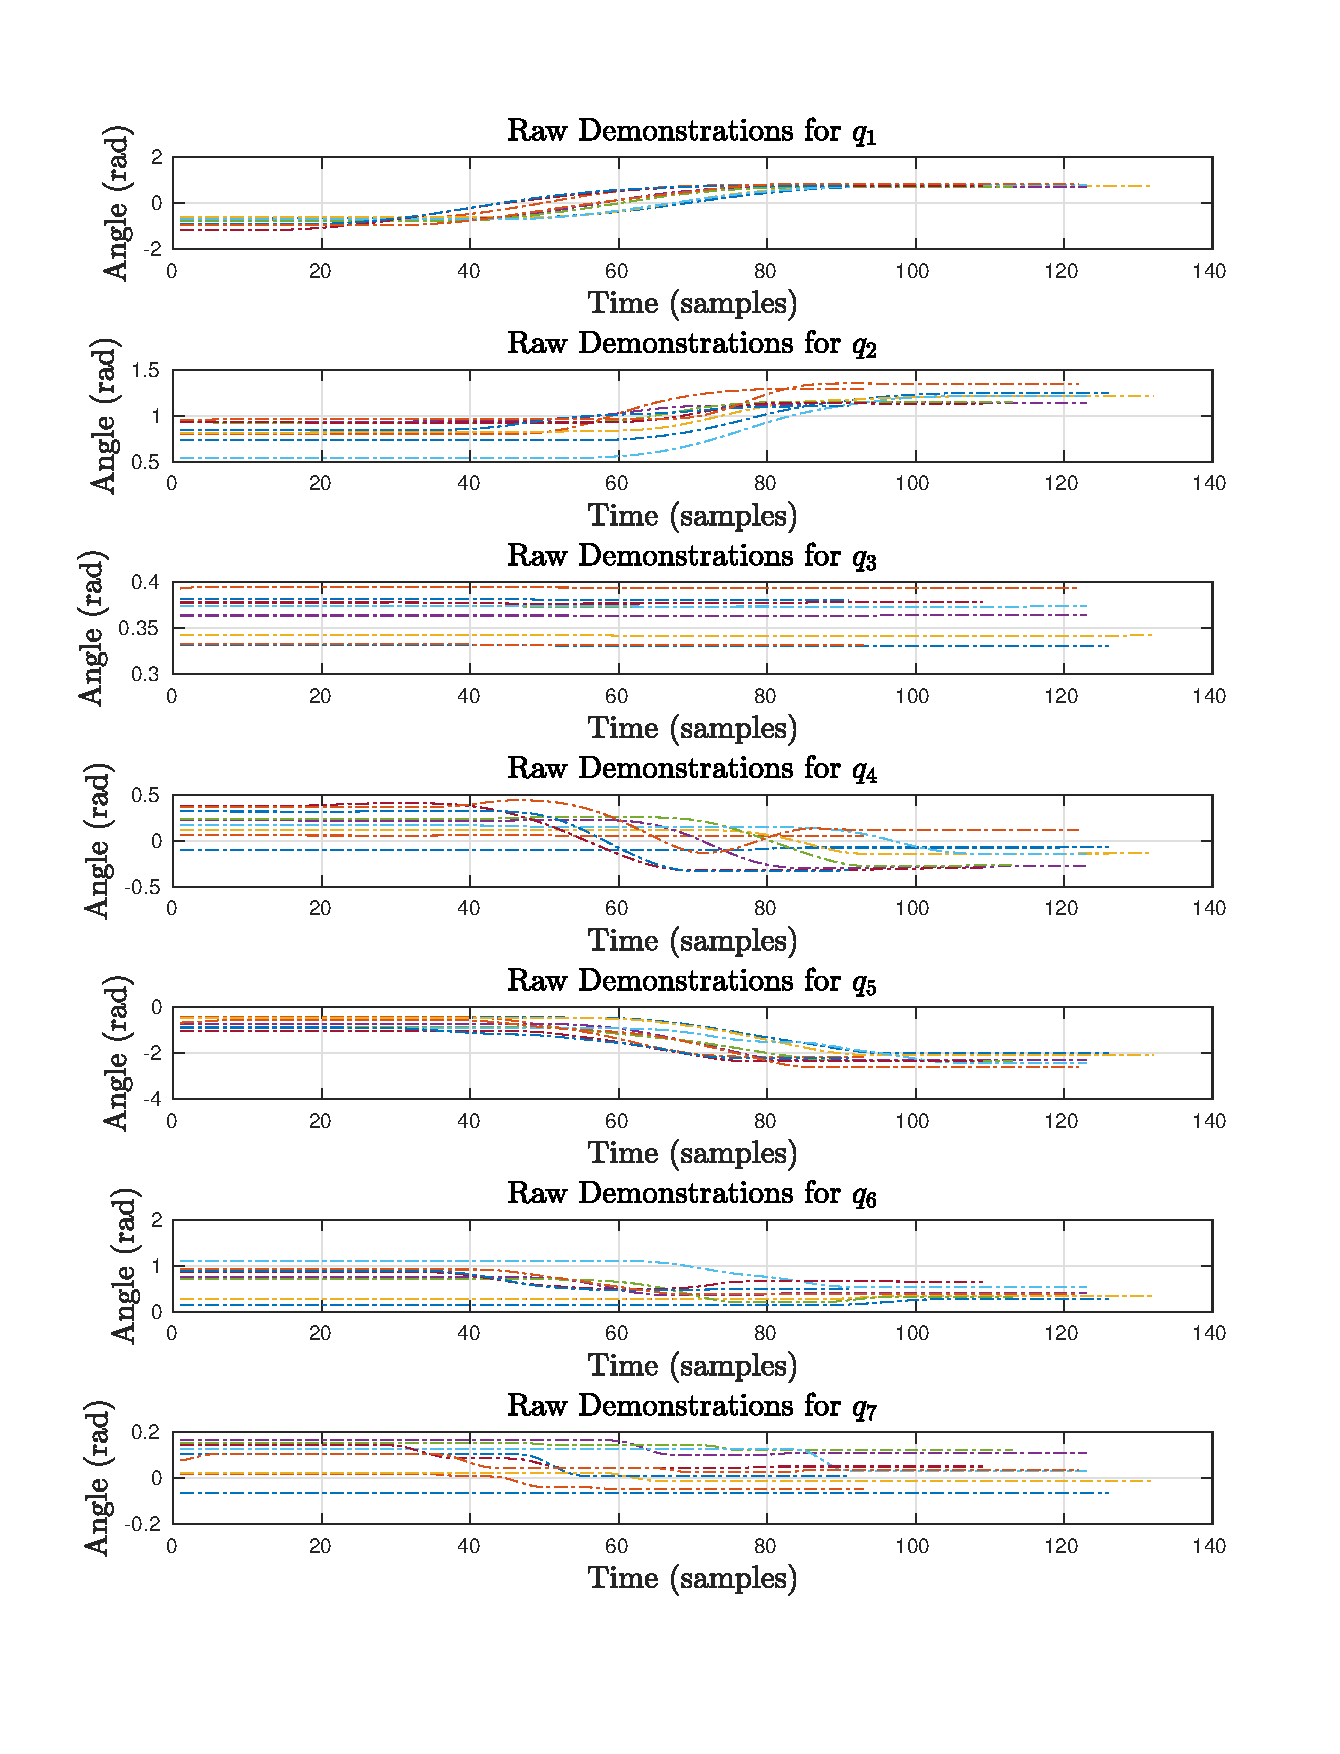
\includegraphics[trim={1.2cm 2cm 1.7cm 2cm},clip,width=\linewidth]{../../src/JTDS_mat_lib/figures/raw_demos_pour.pdf}
  \end{minipage}
   \begin{minipage}{0.47\textwidth}
      	\centering
      	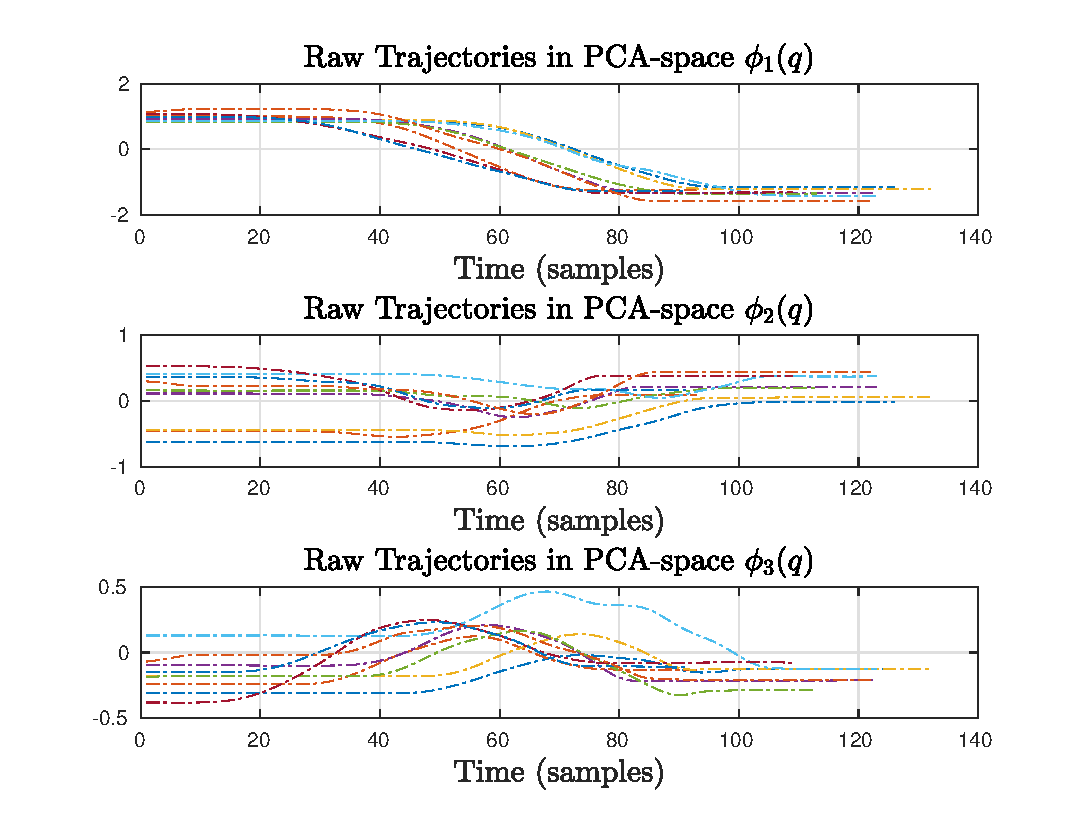
\includegraphics[trim={1.2cm 0.5cm 0.5cm 0.35cm},clip,width=\linewidth]{../../src/JTDS_mat_lib/figures/raw_demos_pca_pour.pdf}
      	\vspace{-5pt}
      	
		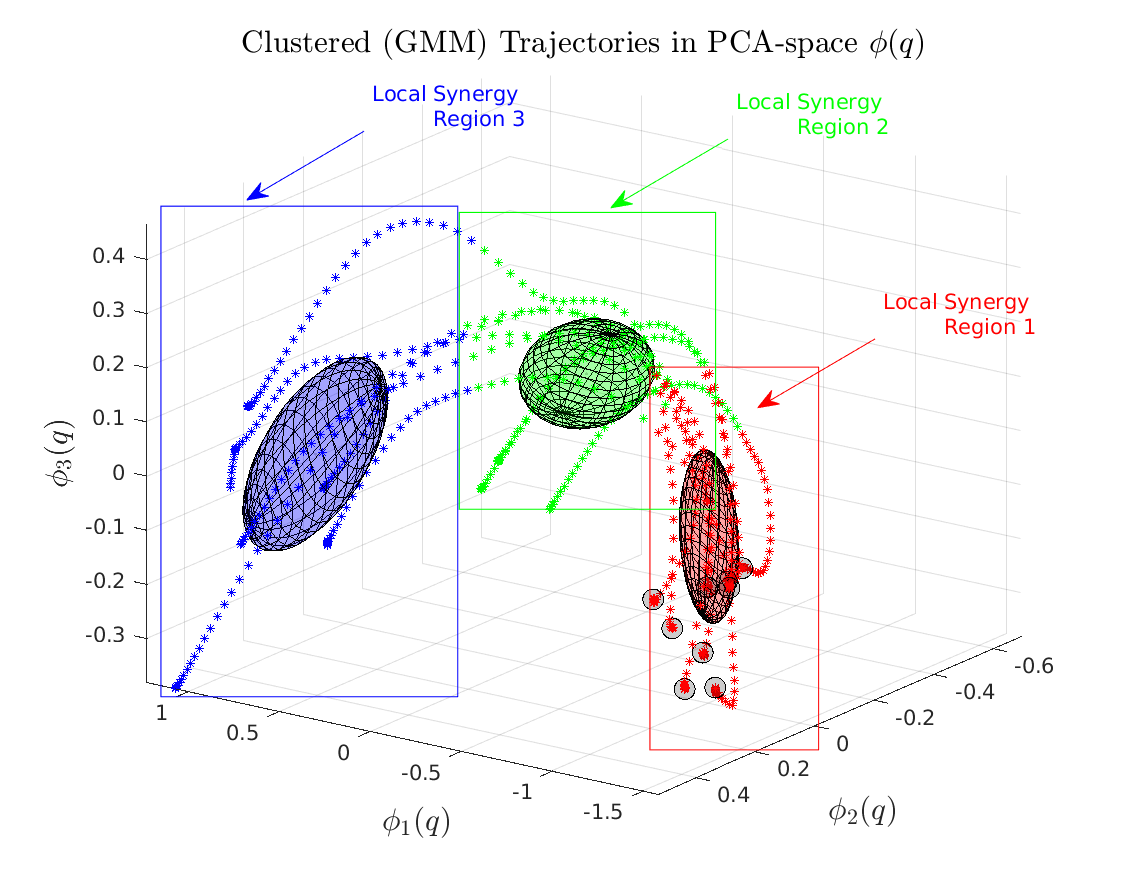
\includegraphics[trim={0.8cm 0.5cm 0cm 0.35cm},clip,width=\linewidth]{../../src/JTDS_mat_lib/figures/local_synergy_regions_pour_annotated.pdf}
   \end{minipage}
   \caption{Raw demonstrations of the pouring task in original space, PCA space and the extracted local synergy regions. \label{fig:raw_demos}}
\end{figure*}

\underline{As mentioned in the reviewers 3rd comment}, since we have an accurate representation of our joint posture trajectories and the local synergy regions in this lower-dimensional space, why not learn the $A_k$ matrices in this space; i.e. $\mathcal{A}(q)\in \mathbb{R}^{p\times p}$ rather than $\mathcal{A}(q)\in \mathbb{R}^{m\times m}$ ? This seems like the obvious method, if we were considering our synergistic approach the classical way, i.e. using the lower-dimensional space as the new control variables. However, if we were to do that, this would mean that \eqref{eq:jtds} would become:
\begin{equation}
\underbrace{\dot{q}}_{\mathbb{R}^{m\times 1}} = -\underbrace{M_p^{-1}}_{\mathbb{R}^{m\times p}}\underbrace{\mathcal{A}(q)}_{\mathbb{R}^{p\times p}}\underbrace{M_p}_{\mathbb{R}^{p\times m}}\underbrace{J^{T}(q)}_{\mathbb{R}^{m\times d}}\underbrace{(H(q)-x^*)}_{\mathbb{R}^{d\times 1}}
\label{eq:jtds_low}
\end{equation}
This is not entirely incorrect, however, with such a control law we can no longer guarantee stability and convergence to the attractor $x^{*}$. By considering the Lyapunov function used in Appendix I to prove stability of \eqref{eq:jtds_low} i.e. $V(q) = \frac{1}{2}(H(q) - x^*)^T(H(q) - x^*)$, the derivative of $ V $ wrt. time with is:
\begin{equation}
\begin{aligned}
\frac{dV(q)}{dt} &= (H(q) - x^*)^TJ(q)\dot{q}\\
&= -(H(q) - x^*)^TJ(q)M_p^{-1}\mathcal{A}(q)M_pJ^T(q)(H(q) - x^*)\\
&= -(H(q) - x^*)^TJ(q)\textcolor{red}{\underbrace{M_p^{-1}\big(\sum_{k=1}^{K}\underbrace{\theta_k(q)}_{> 0}\underbrace{A_k}_{\succ 0}\big)M_p}_{\text{This should be}~~ \succ 0}}J^T(q)(H(q) - x^*)\leq 0
\end{aligned}
\end{equation}
In order for \eqref{eq:jtds_low} to be asymptotically stable wrt. the attractor $x^*$ the term $M_p^{-1}\big(\sum_{k=1}^{K}\theta_k(q)A_k\big)M_p \in \mathbb{R}^{m\times m}$ should undoubtedly be $\succ 0$. Even if $\theta_k(q) > 0$ and $A_k \succ 0$ for all $k$, the only way for this condition to hold is if $M_p$ where a full symmetric positive definite matrix. However, this is not the case because $M_p\in \mathbb{R}^{p\times m}$  is a projection matrix, i.e. $p<m$. The term $M_p^{-1}\big(\sum_{k=1}^{K}\theta_k(q)A_k\big)M_p$ will no longer be full-rank, it will preserve the $p$ positive eigenvalues from the $A_k$ matrices, but the remaining eigenvalues will be 0, thus generating a semi-positive definite matrix, which invalidates our stability proof. Note that, as described in the Appendix, $J(q)$ is not proven to be full rank in all regions of the workspace, when this happens, this means that the end-effector pose is not manipulable. Hence, we can only prove asymptotic stability when the end-effector pose is manipulable. This is a physical artifact from the joint-space constraints of the robot arm which we cannot avoid. Nevertheless, since the demonstrations are acquired via kinesthetic teaching we can assume that all of the regions in task-space are manipulable. Hence, when $M_p^{-1}\big(\sum_{k=1}^{K}\theta_k(q)A_k\big)M_p$ has some eigenvalues $=0$ the physical meaning behind it is that we are loosing control of these DOF of the arm which will restrain us from converging to the attractor and are no longer capable of accurately following the joint-space demonstrations. If instead we learn the synergy matrices in joint-space following \eqref{eq:jtds} and modulate them with the activation function in PCA-space, we avoid this problem of loosing rank altogether. 

\noindent \textbf{Remark 1:} This analysis is only considering PCA as the DR approach. If we would consider K-PCA, deriving such a control law is more involved as the inverse mapping $\phi(q)^{-1}$ is not straightforward.

\noindent \textbf{Remark 2:} If we were to bypass the DR step our state-dependent system matrix would become $\mathcal{A}(q)= \sum\limits_{k=1}^{K}\theta(q)A_k$, which (via our definition) is a combination of ``local behavior synergy matrices" with the activation function living in joint-space rather than the PCA space; known as the \textit{postural synergy space}. The fact that we use PCA/K-PCA to represent the activation function $\theta(\cdot)$ is to alleviate the complexity of extracting the local synergy regions in joint-space directly. It is, indeed, also motivated by the fact that we know that multi-DOF joint postures can be accurately represented in a lower-dimensional space composed of the principal components of the postural trajectories; i.e. the well-known \textit{joint postural synergies}. As shown in TABLE I of the manuscript and discussed in Section V, by using a lower-dimensional manifold to represent the joint trajectories, we are getting rid of outliers, noise and redundancies that might arise from the raw joint demonstrations. Hence, through DR we are capable of robustly extracting the local behavior synergies from raw demonstrations. \\

\noindent \underline{On the applicability of F-PCA to our learning scheme:} ... it is not applicable as we do not want to reconstruct the full trajectory, we only want find the local synergy region that the current joint posture $q$ belongs to.. maybe apply F-PCA to this same demonstration...



%\begin{thebibliography}{9}
%\bibitem[Doe]{doe} \emph{First and last \LaTeX{} example.},
%John Doe 50 B.C. 
%\end{thebibliography}

\end{document}





\end{newlfm}
\end{document}